\documentclass{article}
\usepackage{tikz}
\usepackage{tikz-3dplot}
\usepackage{ifthen}
\usetikzlibrary{calc}
\usepackage{amsmath}
\usepackage{amssymb}
\usetikzlibrary{arrows.meta, decorations.markings}
\usepackage[dvipsnames]{xcolor}
\usepackage[a4paper,margin=10mm]{geometry}
\tdplotsetmaincoords{70}{110}

\colorlet{Xcol}{red}
\colorlet{Ycol}{blue}
\colorlet{Zcol}{Green}

\colorlet{colPsi}{BrickRed}
\colorlet{colTheta}{BlueGreen}
\colorlet{colPhi}{teal}

\def\radius{1.1}
\def\axlen{1.4}
\def\rotpsi{60}
\def\rottheta{50}
\def\ux{cos(\psi)*cos(\theta)}
\def\uy{sin(\psi)*cos(\theta)}
\def\uz{sin(\theta)}

\def\rphi{0.15}
\def\rotphi{60}
\pagenumbering{gobble}
\begin{document}

\begin{tikzpicture}[tdplot_main_coords, scale=3]
  \draw[line width=0.6pt,->, black!30] (0,0,0) -- (\axlen,0,0) node[below left, scale=1.5] {\textcolor{Xcol}{$x$}};
  \draw[line width=0.6pt,->, black!30] (0,0,0) -- (0,\axlen,0) node[right, scale=1.5]  {\textcolor{Ycol}{$y$}};
  \draw[line width=0.6pt,->, black!30] (0,0,0) -- (0,0,\axlen) node[above, scale=1.5]  {\textcolor{Zcol}{$z$}};

  \draw[line width=0.8pt, dashed, black!60] plot[domain=0:360, samples=180] (0, {\radius*cos(\x) * 0.5}, {\radius*sin(\x) * 0.5});
  
  \begin{scope}[
  ]
    \draw[very thick, <-, colPhi] plot[domain=-40:255, samples=180] ({\axlen * 0.4}, {\rphi * cos(\x)}, {\rphi * sin(\x)});
    \node[colPhi, scale=2] at ({\axlen * 0.35}, 0.15, 0.32) {$\varphi$};
    \draw[line width=3pt, line cap=round] (0, 0, 0) -- (\radius, 0, 0);
    \draw[very thick, <-, colPhi] plot[domain=-40:200, samples=180] ({\axlen * 0.4}, {\rphi * cos(\x)}, {\rphi * sin(\x)});
  \end{scope}
\end{tikzpicture}

\begin{tikzpicture}[tdplot_main_coords, scale=3]
  \draw[line width=0.6pt,->, black!30] (0,0,0) -- (\axlen,0,0) node[below left, scale=1.5] {\textcolor{Xcol}{$x$}};
  \draw[line width=0.6pt,->, black!30] (0,0,0) -- (0,\axlen,0) node[right, scale=1.5]  {\textcolor{Ycol}{$y$}};
  \draw[line width=0.6pt,->, black!30] (0,0,0) -- (0,0,\axlen) node[above, scale=1.5]  {\textcolor{Zcol}{$z$}};

  \draw[line width=0.8pt, dashed, black!60] plot[domain=0:360, samples=180] ({\radius*cos(\x)},0, {\radius*sin(\x)});
  
  \begin{scope}[
    rotate around y=-\rottheta
  ]
    \draw[very thick, <-, colPhi] plot[domain=-40:235, samples=180] ({\axlen * 0.4}, {\rphi * cos(\x)}, {\rphi * sin(\x)});
    \node[scale=2] at ({\radius * cos(\rottheta / 2 - 55) * 0.6}, 0, {\radius * sin(\rottheta / 2 - 55) * 0.6}) {\textcolor{colTheta}{$\theta$}};
    \node[colPhi, scale=2] at ({\axlen * 0.35}, 0.15, 0.32) {$\varphi$};
    \draw[line width=3pt, line cap=round] (0, 0, 0) -- (\radius, 0, 0);
    \draw[very thick, colTheta, ->] plot[domain=-\rottheta :0, samples=180] ({\radius * cos(\x)}, 0, {\radius * sin(\x)});
  \end{scope}
  \draw[very thick, colTheta, dashed] (0, 0, 0) -- (\radius, 0, 0);
\end{tikzpicture}

\begin{tikzpicture}[tdplot_main_coords, scale=3]
  \draw[line width=0.6pt,->, black!30] (0,0,0) -- (\axlen,0,0) node[below left, scale=1.5] {\textcolor{Xcol}{$x$}};
  \draw[line width=0.6pt,->, black!30] (0,0,0) -- (0,\axlen,0) node[right, scale=1.5]  {\textcolor{Ycol}{$y$}};
  \draw[line width=0.6pt,->, black!30] (0,0,0) -- (0,0,\axlen) node[above, scale=1.5]  {\textcolor{Zcol}{$z$}};

  \draw[line width=0.8pt, dashed, black!60] plot[domain=0:360, samples=180] ({\radius*cos(\x)},{\radius*sin(\x)}, 0);

  \draw[very thick, colPsi, dashed] (0, 0, 0) -- ({\radius * cos(\rotpsi)}, {\radius * sin(\rotpsi)}, 0);
  \draw[very thick, colPsi, ->] plot[domain=0:\rotpsi, samples=180] ({\radius*cos(\x)},{\radius*sin(\x)}, 0);
  \node[scale=2] at ({\radius * cos(\rotpsi / 2) * 0.6}, {\radius * sin(\rotpsi / 2) * 0.5}, 0) {\textcolor{colPsi}{$\psi$}};
  
  \node[scale=2] at ({\radius * cos(\rotpsi) * cos(\rottheta) * 0.5}, {\radius * sin(\rotpsi) * cos(\rottheta / 2) * 0.6}, {\radius * sin(\rottheta / 2) * 0.5}) {\textcolor{colTheta}{$\theta$}};
  
  \begin{scope}[
    rotate around z=\rotpsi, rotate around y=-\rottheta
  ]
    \draw[very thick, <-, colPhi] plot[domain=-50:235, samples=180] ({\axlen * 0.4}, {\rphi * cos(\x)}, {\rphi * sin(\x)});
    \node[colPhi, scale=2] at ({\axlen * 0.35}, 0.15, 0.32) {$\varphi$};
  \end{scope}

  \draw[line width=3pt, line cap=round] (0, 0, 0) -- ({\radius * cos(\rotpsi) * cos(\rottheta)}, {\radius * sin(\rotpsi) * cos(\rottheta)}, {\radius * sin(\rottheta)});
  \draw[very thick, colTheta, ->] plot[domain=0:\rottheta, samples=180] ({\radius * cos(\rotpsi) * cos(\x)}, {\radius * sin(\rotpsi) * cos(\x)}, {\radius * sin(\x)});
  \begin{scope}[
    rotate around z=\rotpsi, rotate around y=-\rottheta
  ]
    \draw[very thick, colPhi] plot[domain=90:225, samples=180] ({\axlen * 0.4}, {\rphi * cos(\x)}, {\rphi * sin(\x)});
  \end{scope}
\end{tikzpicture}


\vspace{1cm}

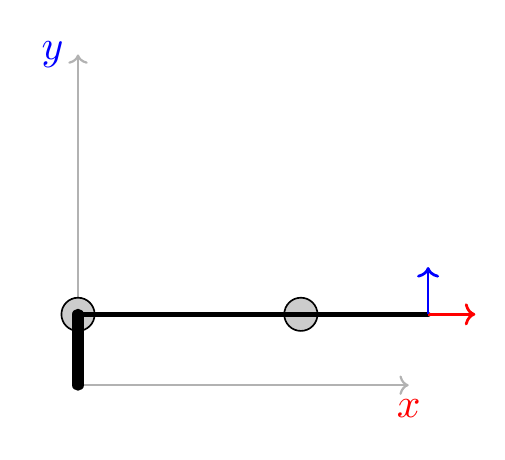
\begin{tikzpicture}[scale=3]
  \draw[line width=0.8pt,->, black!30] (0,0) -- (\axlen,0);
  \draw[line width=0.8pt,->, black!30] (0,0) -- (0,\axlen);

  \node[below, scale=1.5] at (\axlen,0) {\textcolor{Xcol}{$x$}};
  \node[left, scale=1.5] at (0,\axlen) {\textcolor{Ycol}{$y$}};

  \begin{scope}[shift={(0,0.3)}]

    \filldraw[line width=0.6pt, fill=black!20] (0, 0) circle (2pt);
    \filldraw[line width=0.6pt, fill=black!20] (0.9434, 0) circle (2pt);


    \draw[line width=2pt, line cap=round] (0,0) -- (0.9434, 0);
    \draw[line width=2pt, line cap=round] (0.9434, 0) -- ({0.9434 + 0.5385}, 0);

    \begin{scope}[shift={({0.9434 + 0.5385}, 0)}, rotate around z=0]
      \draw[line width=1pt,->, Xcol] (0, 0) -- (0.2, 0);
      \draw[line width=1pt,->, Ycol] (0, 0) -- (0, 0.2);
    \end{scope}
  \end{scope}
  \draw[line width=4pt, line cap=round] (0, 0) -- (0, 0.3);
\end{tikzpicture}

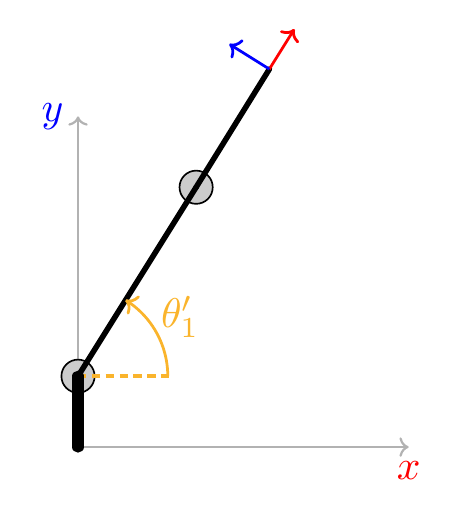
\begin{tikzpicture}[scale=3]
  \draw[line width=0.8pt,->, black!30] (0,0) -- (\axlen,0);
  \draw[line width=0.8pt,->, black!30] (0,0) -- (0,\axlen);

  \node[below, scale=1.5] at (\axlen,0) {\textcolor{Xcol}{$x$}};
  \node[left, scale=1.5] at (0,\axlen) {\textcolor{Ycol}{$y$}};

  \begin{scope}[shift={(0,0.3)}]

    \filldraw[line width=0.6pt, fill=black!20] (0, 0) circle (2pt);
    \filldraw[line width=0.6pt, fill=black!20] (0.5, 0.8) circle (2pt);

    \draw[line width=1.5pt, densely dashed, Dandelion] (0, 0) -- (0.4, 0);

    \draw[line width=2pt, line cap=round] (0,0) -- (0.5, 0.8);
    \draw[line width=2pt, line cap=round] (0.5, 0.8) -- (0.81, 1.3);

    \draw[line width=1pt, Dandelion, ->] plot[domain=90:32, samples=180] ({sin(\x)*0.38}, {cos(\x)*0.38});
    \node[Dandelion, scale=1.5] at ({sin(60)*0.5}, {cos(60)*0.5}) {\textcolor{Dandelion}{$\theta_1'$}};
    \begin{scope}[shift={(0.81, 1.3)}, rotate around z=58]
      \draw[line width=1pt,->, Xcol] (0, 0) -- (0.2, 0);
      \draw[line width=1pt,->, Ycol] (0, 0) -- (0, 0.2);
    \end{scope}
  \end{scope}
  \draw[line width=4pt, line cap=round] (0, 0) -- (0, 0.3);
\end{tikzpicture}

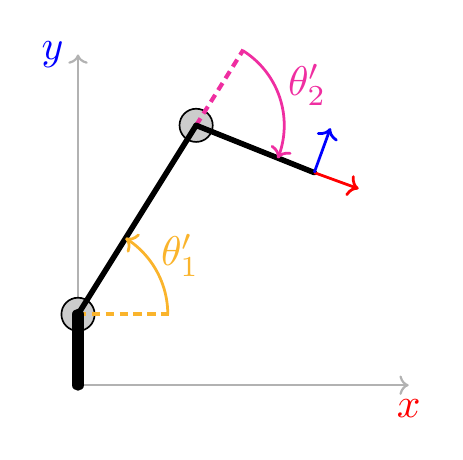
\begin{tikzpicture}[scale=3]
  \draw[line width=0.8pt,->, black!30] (0,0) -- (\axlen,0);
  \draw[line width=0.8pt,->, black!30] (0,0) -- (0,\axlen);

  \node[below, scale=1.5] at (\axlen,0) {\textcolor{Xcol}{$x$}};
  \node[left, scale=1.5] at (0,\axlen) {\textcolor{Ycol}{$y$}};

  \begin{scope}[shift={(0,0.3)}]

    \filldraw[line width=0.6pt, fill=black!20] (0, 0) circle (2pt);
    \filldraw[line width=0.6pt, fill=black!20] (0.5, 0.8) circle (2pt);

    \draw[line width=1.5pt, densely dashed, Dandelion] (0, 0) -- (0.4, 0);
    \draw[line width=1.5pt, densely dashed, Rhodamine] (0.5, 0.8) -- ({0.5 * 1.4}, {0.8 * 1.4});

    \draw[line width=2pt, line cap=round] (0,0) -- (0.5, 0.8);
    \draw[line width=2pt, line cap=round] (0.5, 0.8) -- (1, 0.6);

    \draw[line width=1pt, Dandelion, ->] plot[domain=90:32, samples=180] ({sin(\x)*0.38}, {cos(\x)*0.38});
    \node[Dandelion, scale=1.5] at ({sin(60)*0.5}, {cos(60)*0.5}) {\textcolor{Dandelion}{$\theta_1'$}};
    \draw[line width=1pt, Rhodamine, ->] plot[domain=32:112, samples=180] ({sin(\x)*0.373 + 0.5}, {cos(\x)*0.373 + 0.8});
    \node[Dandelion, scale=1.5] at ({sin(70)*0.5 + 0.5}, {cos(70)*0.5 + 0.8}) {\textcolor{Rhodamine}{$\theta_2'$}};
    \begin{scope}[shift={(1, 0.6)}, rotate around z=-20]
      \draw[line width=1pt,->, Xcol] (0, 0) -- (0.2, 0);
      \draw[line width=1pt,->, Ycol] (0, 0) -- (0, 0.2);
    \end{scope}
  \end{scope}
  \draw[line width=4pt, line cap=round] (0, 0) -- (0, 0.3);
\end{tikzpicture}

\vspace{1cm}
\begin{tikzpicture}[tdplot_main_coords, scale=3]
  \draw[->, black!30] (0,0,0) -- (\axlen,0,0) node[below left, scale=1.5] {\textcolor{Xcol}{$x$}};
  \draw[->, black!30] (0,0,0) -- (0,\axlen,0) node[right, scale=1.5]  {\textcolor{Ycol}{$y$}};
  \draw[->, black!30] (0,0,0) -- (0,0,\axlen) node[above, scale=1.5]  {\textcolor{Zcol}{$z$}};

  \begin{scope}[canvas is yx plane at z=0]
    \filldraw[line width=0.6pt, fill=black!20] (0, 0) circle (0.1);
  \end{scope}

  \begin{scope}[shift={(0,0,0.3)},rotate around z=-20, canvas is yz plane at x=0]
    \filldraw[line width=0.6pt, fill=black!20] (0, 0) circle (0.1);
    \filldraw[line width=0.6pt, fill=black!20] (0.5, 0.8) circle (0.1);
  \end{scope}

  \begin{scope}[shift={(0,0,0.3)}, rotate around z=70]
    \draw[line width=1.2pt, densely dashed, Dandelion] (0,0, 0) -- (0.4,0, 0);
    \draw[line width=1.2pt, densely dashed, Rhodamine] (0.5,0, 0.8) -- ({0.5 * 1.4},0, {0.8 * 1.4});

    \draw[line width=2pt, line cap=round] (0,0,0) -- (0.5,0, 0.8);
    \draw[line width=2pt, line cap=round] (0.5,0, 0.8) -- (1,0, 0.6);

    \draw[line width=1pt, Dandelion,->] plot[domain=90:32, samples=180] ({sin(\x)*0.4},0, {cos(\x)*0.4});
    \node[Dandelion, scale=1.5] at ({sin(60)*0.6},0, {cos(60)*0.6}) {\textcolor{Dandelion}{$\theta_2$}};
    \draw[line width=1pt, Rhodamine,->] plot[domain=32:112, samples=180] ({sin(\x)*0.4 + 0.5},0, {cos(\x)*0.4 + 0.8});
    \node[Dandelion, scale=1.5] at ({sin(65)*0.6 + 0.5},0, {cos(65)*0.6 + 0.8}) {\textcolor{Rhodamine}{$\theta_3$}};

    \begin{scope}[shift={(1,0, 0.6)}, rotate around y=20]
      \draw[line width=1pt,->, Xcol] (0, 0, 0) -- (0.2, 0, 0);
      \draw[line width=1pt,->, Ycol] (0, 0, 0) -- (0, 0.2, 0);
      \draw[line width=1pt,->, Zcol] (0, 0, 0) -- (0, 0, 0.2);
    \end{scope}
  \end{scope}
  
  \draw[line width=4pt, line cap=round] (0, 0, 0) -- (0, 0, 0.3);
  \draw[line width=1.2pt, densely dashed, SeaGreen] (0, 0, 0) -- (0.4,0, 0);
  \draw[line width=1.2pt, densely dashed, SeaGreen] (0, 0, 0) -- ({sin(20)*0.4}, {cos(20)*0.4}, 0);
  \draw[line width=1pt, SeaGreen, <-] plot[domain=20:90, samples=180] ({sin(\x)*0.4}, {cos(\x)*0.4}, 0);
  \node[Dandelion, scale=1.5] at ({sin(60)*0.75}, {cos(60)*0.75}, 0) {\textcolor{SeaGreen}{$\theta_1$}};
  \begin{scope}[shift={(0,0,0.3)}]
    % \draw[line width=0.6pt, densely dashed, SeaGreen!50] (0, 0, 0) -- (0.4,0, 0);
    % \draw[line width=0.5pt, SeaGreen!50, <-] plot[domain=20:90, samples=180] ({sin(\x)*0.4}, {cos(\x)*0.4}, 0);
  \end{scope}

  \begin{scope}[shift={(0,0,1.1)}]
    % \draw[line width=0.6pt, densely dashed, SeaGreen!50] (0, 0, 0) -- (0.5,0, 0);
    % \draw[line width=0.5pt, SeaGreen!50, <-] plot[domain=20:90, samples=180] ({sin(\x)*0.5}, {cos(\x)*0.5}, 0);
  \end{scope}

\end{tikzpicture}

\newpage
\noindent
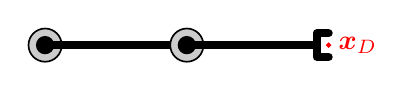
\begin{tikzpicture}[scale=3]
  \filldraw[line width=0.6pt, fill=black!20] (0, 0) circle (2pt);
  \filldraw[line width=0.6pt, fill=black] (0, 0) circle (1pt) ;
  \begin{scope}
    \draw[line width=3pt, line cap=round] (0,0) -- (0.6, 0);
    \filldraw[line width=0.6pt, fill=black!20] (0.6, 0) circle (2pt);
    \filldraw[line width=0.6pt, fill=black] (0.6, 0) circle (1pt);
    \begin{scope}[shift={(0.6, 0)}]
      \draw[line width=3pt, line cap=round] (0,0) -- (0.55, 0);
      \draw[line width=3pt, line cap=round, line join=round] (0.6, -0.05) -- (0.55,-0.05) -- (0.55, 0.05) -- (0.6, 0.05);
      \filldraw[line width=0.6pt, red] (0.6, 0) circle (0.2pt) node[right] {\textcolor{red}{$\boldsymbol{x}_D$}};
    \end{scope}
  \end{scope}
\end{tikzpicture}
\vspace{1cm}
\\
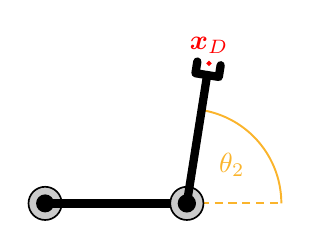
\begin{tikzpicture}[scale=3]
  \filldraw[line width=0.6pt, fill=black!20] (0, 0) circle (2pt);
  \filldraw[line width=0.5pt, fill=black] (0, 0) circle (1pt);
  
  \begin{scope}
    \draw[line width=0.7pt, densely dashed, Dandelion] (0.6,0) -- (1, 0);
    \draw[line width=0.7pt, Dandelion] plot[domain=0:81.0107, samples=180] ({0.4 * cos(\x)+0.6},{0.4 * sin(\x)});
    \node at ({0.25 * cos(81.0107/2)+0.6},{0.25 * sin(81.0107/2)}) {\textcolor{Dandelion}{$\theta_{2}$}};
    \draw[line width=3pt, line cap=round] (0,0) -- (0.6, 0);
    \filldraw[line width=0.6pt, fill=black!20] (0.6, 0) circle (2pt);
    \begin{scope}[shift={(0.6, 0)}, rotate around z=81.0107]
      \draw[line width=3pt, line cap=round] (0,0) -- (0.55, 0);
      \draw[line width=3pt, line cap=round, line join=round] (0.6, -0.05) -- (0.55,-0.05) -- (0.55, 0.05) -- (0.6, 0.05);
      \filldraw[line width=0.6pt, red] (0.6, 0) circle (0.2pt) node[above] {\textcolor{red}{$\boldsymbol{x}_D$}};
    \end{scope}
    \filldraw[line width=0.6pt, fill=black] (0.6, 0) circle (1pt);
  \end{scope}
\end{tikzpicture}
\vspace{1cm}
\\
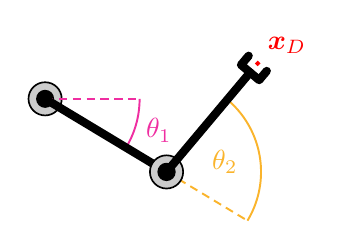
\begin{tikzpicture}[scale=3]
  \filldraw[line width=0.6pt, fill=black!20] (0, 0) circle (2pt);
  \filldraw[line width=0.5pt, fill=black] (0, 0) circle (1pt);
  \draw[line width=0.7pt, densely dashed, Rhodamine] (0,0) -- (0.4, 0);
  \draw[line width=0.7pt, Rhodamine] plot[domain=0:-31.04302, samples=180] ({0.4 * cos(\x)},{0.4 * sin(\x)});
  \node at ({0.5 * cos(-31.04302/2)},{0.5 * sin(-31.04302/2)}) {\textcolor{Rhodamine}{$\theta_{1}$}};
  \begin{scope}[rotate around z=-31.04302]
    \draw[line width=0.7pt, densely dashed, Dandelion] (0.6,0) -- (1, 0);
    \draw[line width=0.7pt, Dandelion] plot[domain=0:81.0107, samples=180] ({0.4 * cos(\x)+0.6},{0.4 * sin(\x)});
    \node at ({0.25 * cos(81.0107/2)+0.6},{0.25 * sin(81.0107/2)}) {\textcolor{Dandelion}{$\theta_{2}$}};
    \draw[line width=3pt, line cap=round] (0,0) -- (0.6, 0);
    \filldraw[line width=0.6pt, fill=black!20] (0.6, 0) circle (2pt);
    \begin{scope}[shift={(0.6, 0)}, rotate around z=81.0107]
      \draw[line width=3pt, line cap=round] (0,0) -- (0.55, 0);
      \draw[line width=3pt, line cap=round, line join=round] (0.6, -0.05) -- (0.55,-0.05) -- (0.55, 0.05) -- (0.6, 0.05);
      \filldraw[line width=0.6pt, red] (0.6, 0) circle (0.2pt) node[above right] {\textcolor{red}{$\boldsymbol{x}_D$}};
    \end{scope}
    \filldraw[line width=0.6pt, fill=black] (0.6, 0) circle (1pt);
  \end{scope}
\end{tikzpicture}
\\\vspace{2cm}

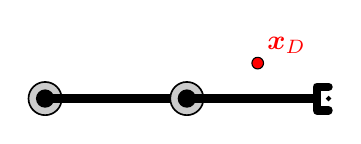
\begin{tikzpicture}[scale=3]
  \filldraw[line width=0.4pt, fill=red] (0.9, 0.15) circle (0.7pt) node[above right] {\textcolor{red}{$\boldsymbol{x}_D$}};
  \filldraw[line width=0.6pt, fill=black!20] (0, 0) circle (2pt);
  \filldraw[line width=0.6pt, fill=black] (0, 0) circle (1pt) ;
  \begin{scope}
    \draw[line width=3pt, line cap=round] (0,0) -- (0.6, 0);
    \filldraw[line width=0.6pt, fill=black!20] (0.6, 0) circle (2pt);
    \filldraw[line width=0.6pt, fill=black] (0.6, 0) circle (1pt);
    \begin{scope}[shift={(0.6, 0)}]
      \draw[line width=3pt, line cap=round] (0,0) -- (0.55, 0);
      \draw[line width=3pt, line cap=round, line join=round] (0.6, -0.05) -- (0.55,-0.05) -- (0.55, 0.05) -- (0.6, 0.05);
      \filldraw[line width=0.6pt, fill=black] (0.6, 0) circle (0.2pt);
    \end{scope}
  \end{scope}
\end{tikzpicture}
\vspace{1cm}
\\
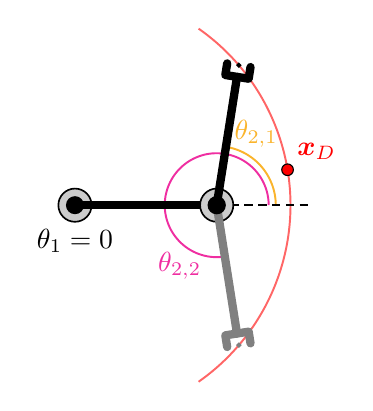
\begin{tikzpicture}[scale=3]
  \draw[line width=0.7pt, red!60] plot[domain=-55:55, samples=180] ({0.912414 * cos(\x)},{0.912414 * sin(\x)});
  \filldraw[line width=0.4pt, fill=red] (0.9, 0.15) circle (0.7pt) node[above right] {\textcolor{red}{$\boldsymbol{x}_D$}};
  \filldraw[line width=0.6pt, fill=black!20] (0, 0) circle (2pt) node[below=5pt] {$\theta_1 = 0$};
  \filldraw[line width=0.5pt, fill=black] (0, 0) circle (1pt);

  \draw[line width=0.7pt, Dandelion] plot[domain=0:81.0107, samples=180] ({0.25 * cos(\x) + 0.6},{0.25 * sin(\x)});
  \draw[line width=0.7pt, Rhodamine] plot[domain=0:{360-81.0107}, samples=180] ({0.22 * cos(\x) + 0.6},{0.22 * sin(\x)});
  \node at ({0.22 * cos(81.0107/2) + 0.6},{0.22 * sin(81.0107/2) + 0.16}) {\textcolor{Dandelion}{$\theta_{2,1}$}};
  \node at ({0.3 * cos(360-81.0107-81.0107/2) + 0.6},{0.3 * sin(360-81.0107-81.0107/2)}) {\textcolor{Rhodamine}{$\theta_{2,2}$}};
  \draw[line width=0.7pt, densely dashed] (0.6,0) -- (1, 0);
  \begin{scope}
    \draw[line width=3pt, line cap=round] (0,0) -- (0.6, 0);
    \filldraw[line width=0.6pt, fill=black!20] (0.6, 0) circle (2pt);
    \begin{scope}[shift={(0.6, 0)}, rotate around z=81.0107]
      \begin{scope}[rotate around z=- {2 * 81.0107}]
        \draw[line width=3pt, line cap=round, gray] (0,0) -- (0.55, 0);
        \draw[line width=3pt, line cap=round, line join=round, gray] (0.6, -0.05) -- (0.55,-0.05) -- (0.55, 0.05) -- (0.6, 0.05);
        \filldraw[line width=0.6pt, fill=black, gray] (0.6, 0) circle (0.2pt);
      \end{scope}
      \draw[line width=3pt, line cap=round] (0,0) -- (0.55, 0);
      \draw[line width=3pt, line cap=round, line join=round] (0.6, -0.05) -- (0.55,-0.05) -- (0.55, 0.05) -- (0.6, 0.05);
      \filldraw[line width=0.6pt, fill=black] (0.6, 0) circle (0.2pt);
    \end{scope}
    \filldraw[line width=0.6pt, fill=black] (0.6, 0) circle (1pt);
  \end{scope}
\end{tikzpicture}
\vspace{1cm}
\\
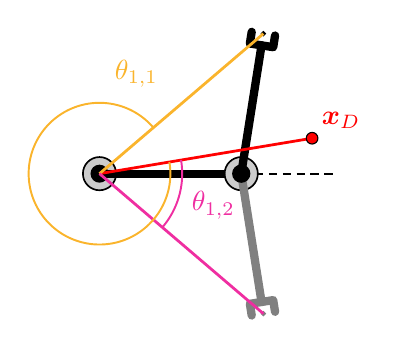
\begin{tikzpicture}[scale=3]
  \filldraw[line width=0.6pt, fill=black!20] (0, 0) circle (2pt);
  \filldraw[line width=0.5pt, fill=black] (0, 0) circle (1pt);
  \node at ({0.45 * cos((180-40.50535)/2)},{0.45 * sin((180-40.50535)/2)}) {\textcolor{Dandelion}{$\theta_{1,1}$}};
  \node at ({0.5 * cos((9.46232-40.50535)/2)},{0.5 * sin((9.46232-40.50535)/2)}) {\textcolor{Rhodamine}{$\theta_{1,2}$}};
  \draw[line width=0.7pt, densely dashed] (0.6,0) -- (1, 0);
  \begin{scope}
    \draw[line width=3pt, line cap=round] (0,0) -- (0.6, 0);
    \filldraw[line width=0.6pt, fill=black!20] (0.6, 0) circle (2pt);
    \begin{scope}[shift={(0.6, 0)}, rotate around z=81.0107]
      \begin{scope}[rotate around z=- {2 * 81.0107}]
        \draw[line width=3pt, line cap=round, gray] (0,0) -- (0.55, 0);
        \draw[line width=3pt, line cap=round, line join=round, gray] (0.6, -0.05) -- (0.55,-0.05) -- (0.55, 0.05) -- (0.6, 0.05);
        \filldraw[line width=0.6pt, fill=black, gray] (0.6, 0) circle (0.2pt);
      \end{scope}
      \draw[line width=3pt, line cap=round] (0,0) -- (0.55, 0);
      \draw[line width=3pt, line cap=round, line join=round] (0.6, -0.05) -- (0.55,-0.05) -- (0.55, 0.05) -- (0.6, 0.05);
      \filldraw[line width=0.6pt, fill=black] (0.6, 0) circle (0.2pt);
    \end{scope}
    \filldraw[line width=0.6pt, fill=black] (0.6, 0) circle (1pt);
  \end{scope}
  \draw[line width=1pt, red] (0, 0) -- (0.9, 0.15);
  \draw[line width=1pt, Dandelion] (0, 0) -- ({0.6 + 0.6 * cos(81.0107)}, {0.6 * sin(81.0107)});
  \draw[line width=1pt, Rhodamine] (0, 0) -- ({0.6 + 0.6 * cos(-81.0107)}, {0.6 * sin(-81.0107)});
  \filldraw[line width=0.4pt, fill=red] (0.9, 0.15) circle (0.7pt) node[above right] {\textcolor{red}{$\boldsymbol{x}_D$}};
  \draw[line width=0.7pt, Dandelion] plot[domain=9.46232:-360+40.50535, samples=180] ({0.3 * cos(\x)},{0.3 * sin(\x)});
  \draw[line width=0.7pt, Rhodamine] plot[domain=9.46232:-40.50535, samples=180] ({0.35 * cos(\x)},{0.35 * sin(\x)});
\end{tikzpicture}
\begin{align*}
  L_n = \left[\begin{matrix}
  L_{n,x}\\
  L_{n,y}\\
  L_{n,z}
  \end{matrix}\right]
\end{align*}
\begin{align*}
  R(\theta) = \left[\begin{matrix}
  \cos{\theta}&-\sin{\theta}\\
  \sin{\theta}&\cos{\theta}
  \end{matrix}\right]
\end{align*}
\begin{align*}
    X_D & =L_1 + R\left(\theta_1\right)L_2+R\left(\theta_1 + \theta_2\right)L_3\\
    X_D & =R\left(\theta_1\right)\left(L_1 + R\left(\theta_2\right)L_2\right)
\end{align*}
\begin{align*}
  x, y, z, \psi, \theta, \phi \longrightarrow \theta_1, \theta_2, \theta_3, \theta_4, \theta_5, \theta_6\\
  \theta_1, \theta_2, \theta_3, \theta_4, \theta_5, \theta_6 \longrightarrow x, y, z, \psi, \theta, \phi \\
\end{align*}
\end{document}